\def\mytitle{ASSIGNMENT} 
\def\myauthor{M Goutham}
\def\contact{mannemahesh327@gmail.com}
\def\mymodule{Future Wireless Communications (FWC)}
\documentclass[journal,12pt]{article}
\usepackage{setspace}
\usepackage{gensymb}
\usepackage{xcolor}
\usepackage{caption}
\usepackage[hyphens,spaces,obeyspaces]{url}
\usepackage[cmex10]{amsmath}
\usepackage{mathtools}
\singlespacing
\usepackage{amsthm}
\usepackage{mathrsfs}
\usepackage{txfonts}
\usepackage{stfloats}
\usepackage{cite}
\usepackage{cases}
\usepackage{subfig}
\usepackage{longtable}
\usepackage{multirow}
\usepackage{graphicx}
\graphicspath{{./images/}}
\usepackage[colorlinks,linkcolor={black},citecolor={blue!80!black},urlcolor={blue!80!black}]{hyperref}
\usepackage[parfill]{parskip}
\usepackage{lmodern}
\usepackage{tikz}
\usepackage{circuitikz}
\usepackage{karnaugh-map}
\usepackage{pgf}
\usepackage[hyphenbreaks]{breakurl}
\usepackage{tabularx}
\usetikzlibrary{calc}
\renewcommand*\familydefault{\sfdefault}
\usepackage{watermark}
\usepackage{lipsum}
\usepackage{xcolor}
\usepackage{listings}
\usepackage{float}
\usepackage{titlesec}
\DeclareMathOperator*{\Res}{Res}
\renewcommand\thesection{\arabic{section}}
\renewcommand\thesubsection{\thesection.\arabic{subsection}}
\renewcommand\thesubsubsection{\thesubsection.\arabic{subsubsection}}

\usetikzlibrary{arrows,shapes,automata,petri,positioning,calc}
\usetikzlibrary{shapes.geometric}
\lstset{
 language=C++,
 basicstyle=\ttfamily\footnotesize,
 breaklines=true,
 frame=lines
 }

% correct bad hyphenation here
\hyphenation{op-tical net-works semi-conduc-tor}

\titlespacing{\subsection}{1pt}{\parskip}{3pt}
\titlespacing{\subsubsection}{0pt}{\parskip}{-\parskip}
\titlespacing{\paragraph}{0pt}{\parskip}{\parskip}
\newcommand{\figuremacro}[5]{
\begin{figure}[#1]
\centering
\includegraphics[width=#5\columnwidth]{#2}
\caption[#3]{\textbf{#3}#4}
\label{fig:#2}
\end{figure}
}
\lstset{
frame=single, 
breaklines=true,
columns=fullflexible
}
\title{\mytitle}
\author{\myauthor\hspace{1em}\\\contact\\IITH\hspace{0.5em}-\hspace{0.6em}\mymodule}
\date{20-07-2023}
\def\inputGnumericTable{}                
\lstset{
frame=single,
breaklines=true,
columns=fullflexible
}
\begin{document}
\theoremstyle{definition}
\newtheorem{theorem}{Theorem}[section]
\newtheorem{problem}{Problem}
\newtheorem{proposition}{Proposition}[section]
\newtheorem{lemma}{Lemma}[section]
\newtheorem{corollary}[theorem]{Corollary}
\newtheorem{example}{Example}[section]
\newtheorem{definition}{Definition}[section]
\newcommand{\BEQA}{\begin{eqnarray}}
\newcommand{\EEQA}{\end{eqnarray}}
\newcommand{\define}{\stackrel{\triangle}{=}}
\bibliographystyle{article}
\vspace{3cm}
\maketitle
\tableofcontents
\pagebreak
\section{Question}
\begin{enumerate}
    \item The circuit shown in the figure below uses ideal positive edge-triggered synchronous J-K flip flops with outputs X and Y. If the initial state of the output is X=0 and Y=0 just before the arrival of the first clock pulse, the state of the output just before the arrival of the second clock pulse is
\end{enumerate}
\begin{figure}[h]
        \centering
	
 \begin{tikzpicture}
        \draw (2,2) rectangle (5,5);            
        \draw (2.5,2.7) node{$K$};
        \draw (2.5,3.7) node{$clk1$};
        \draw[->] (1.6,3.7) -- (2,3.7) node[left] {};%connection of clock 1 
        \draw (2.5,4.5) node{$J$};
        \draw (2,2.7) -- (1,2.7); % this is the connection K
        \draw (0.7,2.7) node{$1$}; % 1 is the given value of K
        \draw (2,4.5) -- (1,4.5); % this the connection of J
        \draw (0.7,4.5) node{$1$}; % 1 is the given value of J
        \draw (5,4) -- (5.75,4);     
        \draw (5.75,4) -- (5.75,3.5);
        \draw (3.5,3.6) node{$FF1$};
        \draw[->] (5.75,3.5) -- (7,3.5) node[left] {};% clock pulse from Q1 to FF2's clock
        \draw (10,4) -- (10.5,4); % this is the connection from Q2
        \draw (5.5,4) -- (5.5,5.6);
        \draw (5.5,5.6) -- (12,5.6);
        \draw (12,5.6) -- (12,3); % this the connection of Y
        \draw (11.99,2.8) node{$Y$}; % this is the co-ordinates Y 
        \draw (10.5,4) -- (10.5,3); %this the line of X
        \draw (10.4,2.8) node{$X$}; %this is co-ordinates of X
        \draw (4.5,4) node{$Q$}; % FF1's Q1
        \draw (7,2) rectangle (10,5);       
        \draw (7.5,2.7) node{$K$};   
        \draw (7,2.7) -- (6.59,2.7); % this the connection of k of FF2
        \draw (6.4,2.7) node{$1$}; % 1 is the given value of K of FF2
        \draw (7.5,3.7) node{$clk$}; 
        \draw (8.6,3.7) node{$FF2$};
        \draw (7.5,4.5) node{$J$};
        \draw (6.4,4.5) node{$1$};
        \draw (7,4.5) -- (6.6,4.5); % this the connection of J of FF2
        \draw (9.5,4) node{$Q$};
        
        
\end{tikzpicture}
  


	\caption{}
\end{figure}
\begin{enumerate}
    \item $X=0, Y=0$
    \item $X=0, Y=1$
    \item $X=1, Y=0$
    \item $X=1, Y=1$
\end{enumerate}
\section{Components}
\begin{table}[h]
\centering
\begin{tabular}{|c|c|c|}
\hline
  \textbf{Component}& \textbf{values} & \textbf{Qantity}\\
\hline
  Arduino & UNO & 1 \\
\hline
  Jumperwires & M-M & 12 \\
\hline
  Breadboard & & 1 \\
\hline
  LED & & 2\\
\hline
  Resistor & 220ohms & 2 \\
\hline
  IC & 7476 & 2 \\
\hline
\end{tabular}
\end{table}
\begin{center}
Figure.a
\end{center}
\section{TruthTable}
\centering
\begin{tabularx}{0.8\textwidth} {
                | >{\centering\arraybackslash}X
                | >{\centering\arraybackslash}X
                | >{\centering\arraybackslash}X
                | >{\centering\arraybackslash}X
                | >{\centering\arraybackslash}X
                | >{\centering\arraybackslash}X | }
\hline
 \textbf{CLK} & \textbf{J} & \textbf{K} & \textbf{Q} & \textbf{Q'} & \textbf{State}\\
\hline
1 & 0 & 0 & Q & Q' & No Change \\
\hline
1 & 0 & 1 & 0 & 1 & Resets Q to 0 \\
\hline
1 & 1 & 0 & 1 & 0 & Sets Q to 1 \\
\hline
1 & 1 & 1 & Q' & Q & Toggle \\
\hline
\end{tabularx}
\begin{center}
Truth tabel of JK filp flop
\end{center}

\section{Stages}
\subsection{Stage 1}
\begin{figure}[h]
	\centering
	 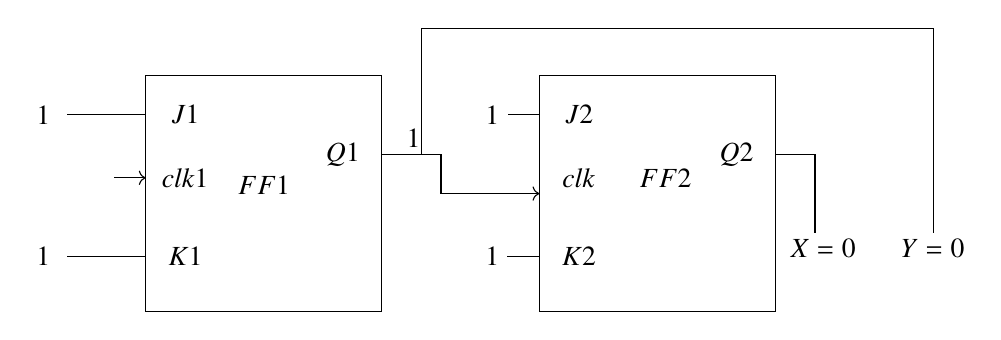
\begin{tikzpicture}
        \draw (2,2) rectangle (5,5);            
        \draw (2.5,2.7) node{$K1$};
        \draw (2.5,3.7) node{$clk1$};
        \draw[->] (1.6,3.7) -- (2,3.7) node[left] {};%connection of clock 1 
        \draw (2.5,4.5) node{$J1$};
        \draw (2,2.7) -- (1,2.7); % this is the connection K
        \draw (0.7,2.7) node{$1$}; % 1 is the given value of K
        \draw (2,4.5) -- (1,4.5); % this the connection of J
        \draw (0.7,4.5) node{$1$}; % 1 is the given value of J
        \draw (5,4) -- (5.75,4);     
        \draw (5.75,4) -- (5.75,3.5);
        \draw (3.5,3.6) node{$FF1$};
        \draw[->] (5.75,3.5) -- (7,3.5) node[left] {};% clock pulse from Q1 to FF2's clock
        \draw (10,4) -- (10.5,4); % this is the connection from Q2
        \draw (5.5,4) -- (5.5,5.6);
        \draw (5.5,5.6) -- (12,5.6);
        \draw (12,5.6) -- (12,3); % this the connection of Y
        \draw (11.99,2.8) node{$Y=0$}; % this is the co-ordinates Y 
        \draw (10.5,4) -- (10.5,3); %this the line of X
        \draw (10.6,2.8) node{$X=0$}; %this is co-ordinates of X
        \draw (4.5,4) node{$Q1$}; % FF1's Q1
        \draw (5.4,4.2) node{$1$}; % 1 is the value of Q1
        \draw (7,2) rectangle (10,5);       
        \draw (7.5,2.7) node{$K2$};   
        \draw (7,2.7) -- (6.59,2.7); % this the connection of k of FF2
        \draw (6.4,2.7) node{$1$}; % 1 is the given value of K of FF2
        \draw (7.5,3.7) node{$clk$}; 
        \draw (8.6,3.7) node{$FF2$};
        \draw (7.5,4.5) node{$J2$};
        \draw (6.4,4.5) node{$1$};
        \draw (7,4.5) -- (6.6,4.5); % this the connection of J of FF2
        \draw (9.5,4) node{$Q2$};
        
        
\end{tikzpicture}
  


	\caption{}
\end{figure}
Initially, let X=0 and Y=0. According to the truth table, when J=1 and K=1, the circuit enters the toggle condition. Given that the previous value of Q1 was 0, toggling it changes Q1 to 1, as illustrated in Figure 2.
\pagebreak
\subsection{stage 2}
\begin{figure}[h]
        \centering
	 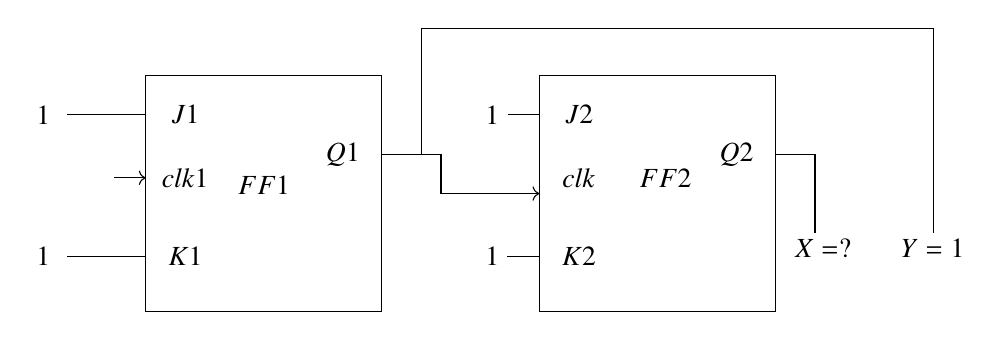
\begin{tikzpicture}
        \draw (2,2) rectangle (5,5);            
        \draw (2.5,2.7) node{$K1$};
        \draw (2.5,3.7) node{$clk1$};
        \draw[->] (1.6,3.7) -- (2,3.7) node[left] {};%connection of clock 1 
        \draw (2.5,4.5) node{$J1$};
        \draw (2,2.7) -- (1,2.7); % this is the connection K
        \draw (0.7,2.7) node{$1$}; % 1 is the given value of K
        \draw (2,4.5) -- (1,4.5); % this the connection of J
        \draw (0.7,4.5) node{$1$}; % 1 is the given value of J
        \draw (5,4) -- (5.75,4);     
        \draw (5.75,4) -- (5.75,3.5);
        \draw (3.5,3.6) node{$FF1$};
        \draw[->] (5.75,3.5) -- (7,3.5) node[left] {};% clock pulse from Q1 to FF2's clock
        \draw (10,4) -- (10.5,4); % this is the connection from Q2
        \draw (5.5,4) -- (5.5,5.6);
        \draw (5.5,5.6) -- (12,5.6);
        \draw (12,5.6) -- (12,3); % this the connection of Y
        \draw (11.99,2.8) node{$Y=1$}; % this is the co-ordinates Y 
        \draw (10.5,4) -- (10.5,3); %this the line of X
        \draw (10.6,2.8) node{$X=?$}; %this is co-ordinates of X
        \draw (4.5,4) node{$Q1$}; % FF1's Q1
        \draw (7,2) rectangle (10,5);       
        \draw (7.5,2.7) node{$K2$};   
        \draw (7,2.7) -- (6.59,2.7); % this the connection of k of FF2
        \draw (6.4,2.7) node{$1$}; % 1 is the given value of K of FF2
        \draw (7.5,3.7) node{$clk$}; 
        \draw (8.6,3.7) node{$FF2$};
        \draw (7.5,4.5) node{$J2$};
        \draw (6.4,4.5) node{$1$};
        \draw (7,4.5) -- (6.6,4.5); % this the connection of J of FF2
        \draw (9.5,4) node{$Q2$};
        
        
\end{tikzpicture}
  

	\caption{}
\end{figure}
After toggling, the value of Q1 is set to be the same as the output value of Y, which is found to be 1. Therefore, both Q1 and Y are equal to 1 after the toggle operation. This behavior occurs due to the specific input conditions (j=1 and k=1) applied to the circuit, as shown in Figure 3
\subsection{stage 3}
\begin{figure}[h]
	\centering
	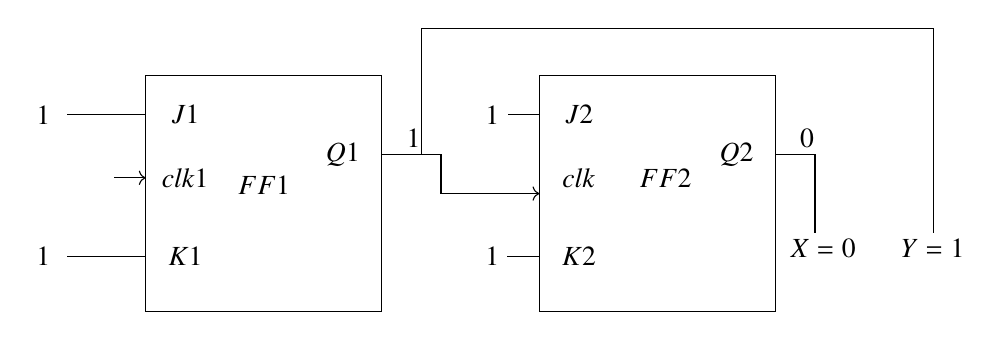
\begin{tikzpicture}
        \draw (2,2) rectangle (5,5);            
        \draw (2.5,2.7) node{$K1$};
        \draw (2.5,3.7) node{$clk1$};
        \draw[->] (1.6,3.7) -- (2,3.7) node[left] {};%connection of clock 1 
        \draw (2.5,4.5) node{$J1$};
        \draw (2,2.7) -- (1,2.7); % this is the connection K
        \draw (0.7,2.7) node{$1$}; % 1 is the given value of K
        \draw (2,4.5) -- (1,4.5); % this the connection of J
        \draw (0.7,4.5) node{$1$}; % 1 is the given value of J
        \draw (5,4) -- (5.75,4);     
        \draw (5.75,4) -- (5.75,3.5);
        \draw (3.5,3.6) node{$FF1$};
        \draw[->] (5.75,3.5) -- (7,3.5) node[left] {};% clock pulse from Q1 to FF2's clock
        \draw (10,4) -- (10.5,4); % this is the connection from Q2
        \draw (5.5,4) -- (5.5,5.6);
        \draw (5.5,5.6) -- (12,5.6);
        \draw (12,5.6) -- (12,3); % this the connection of Y
        \draw (11.99,2.8) node{$Y=1$}; % this is the co-ordinates Y 
        \draw (10.5,4) -- (10.5,3); %this the line of X
        \draw (10.6,2.8) node{$X=0$}; %this is co-ordinates of X
        \draw (4.5,4) node{$Q1$}; % FF1's Q1
        \draw (5.4,4.2) node{$1$}; % 1 is the value of Q1
        \draw (7,2) rectangle (10,5);       
        \draw (7.5,2.7) node{$K2$};   
        \draw (7,2.7) -- (6.59,2.7); % this the connection of k of FF2
        \draw (6.4,2.7) node{$1$}; % 1 is the given value of K of FF2
        \draw (7.5,3.7) node{$clk$}; 
        \draw (8.6,3.7) node{$FF2$};
        \draw (7.5,4.5) node{$J2$};
        \draw (6.4,4.5) node{$1$};
        \draw (7,4.5) -- (6.6,4.5); % this the connection of J of FF2
        \draw (9.5,4) node{$Q2$};
        \draw (10.4,4.2) node{$0$};
        
        
\end{tikzpicture}

	\caption{}
\end{figure}
After Q1 and Y are set to 1, the value of X remains 0. At this point, Q1 is connected as the clock input to Flip Flop 2, causing the second Flip Flop to also enter the toggling condition.
\pagebreak
\subsection{stage 4}
\begin{figure}[h]
	\centering
	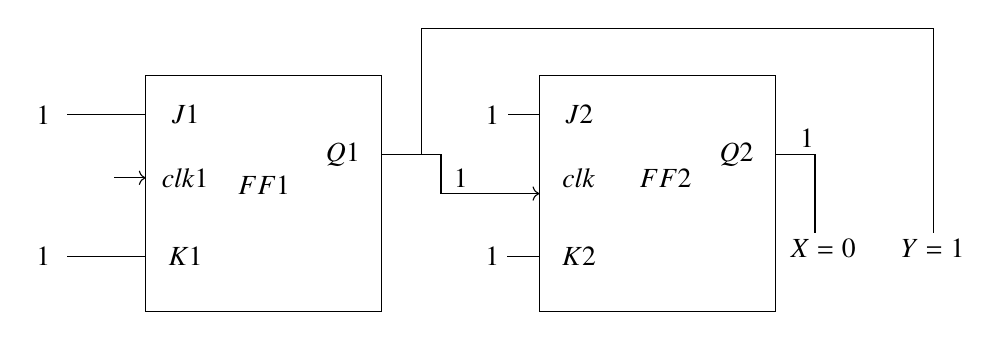
\begin{tikzpicture}
        \draw (2,2) rectangle (5,5);            
        \draw (2.5,2.7) node{$K1$};
        \draw (2.5,3.7) node{$clk1$};
        \draw[->] (1.6,3.7) -- (2,3.7) node[left] {};%connection of clock 1 
        \draw (2.5,4.5) node{$J1$};
        \draw (2,2.7) -- (1,2.7); % this is the connection K
        \draw (0.7,2.7) node{$1$}; % 1 is the given value of K
        \draw (2,4.5) -- (1,4.5); % this the connection of J
        \draw (0.7,4.5) node{$1$}; % 1 is the given value of J
        \draw (5,4) -- (5.75,4);     
        \draw (5.75,4) -- (5.75,3.5);
        \draw (3.5,3.6) node{$FF1$};
        \draw[->] (5.75,3.5) -- (7,3.5) node[left] {};% clock pulse from Q1 to FF2's clock
        \draw (10,4) -- (10.5,4); % this is the connection from Q2
        \draw (5.5,4) -- (5.5,5.6);
        \draw (5.5,5.6) -- (12,5.6);
        \draw (12,5.6) -- (12,3); % this the connection of Y
        \draw (11.99,2.8) node{$Y=1$}; % this is the co-ordinates Y 
        \draw (10.5,4) -- (10.5,3); %this the line of X
        \draw (10.6,2.8) node{$X=0$}; %this is co-ordinates of X
        \draw (4.5,4) node{$Q1$}; % FF1's Q1
        \draw (6,3.7 ) node{$1$}; % 1 is the value of Q1
        \draw (7,2) rectangle (10,5);       
        \draw (7.5,2.7) node{$K2$};   
        \draw (7,2.7) -- (6.59,2.7); % this the connection of k of FF2
        \draw (6.4,2.7) node{$1$}; % 1 is the given value of K of FF2
        \draw (7.5,3.7) node{$clk$}; 
        \draw (8.6,3.7) node{$FF2$};
        \draw (7.5,4.5) node{$J2$};
        \draw (6.4,4.5) node{$1$};
        \draw (7,4.5) -- (6.6,4.5); % this the connection of J of FF2
        \draw (9.5,4) node{$Q2$};
        \draw (10.4,4.2) node{$1$};
\end{tikzpicture}

	\caption{}
\end{figure}
Once Q2 is set to 1, it assumes the same value as X, leading X to automatically become 1 as a result.
\subsection{stage 5}
\begin{figure}[h]
	\centering
	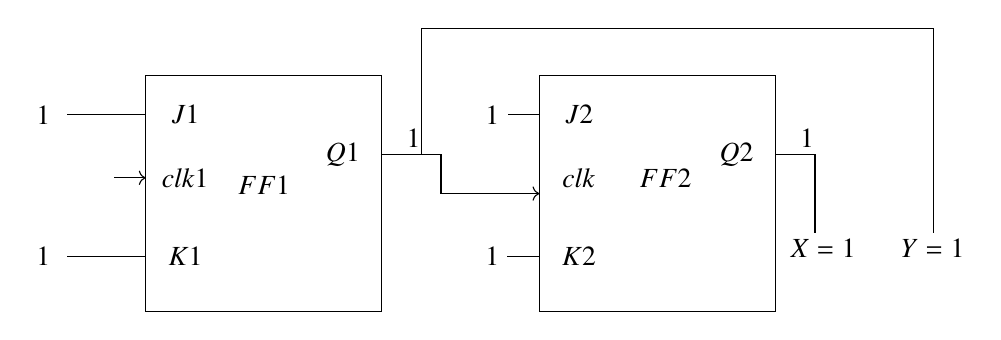
\begin{tikzpicture}
        \draw (2,2) rectangle (5,5);            
        \draw (2.5,2.7) node{$K1$};
        \draw (2.5,3.7) node{$clk1$};
        \draw[->] (1.6,3.7) -- (2,3.7) node[left] {};%connection of clock 1 
        \draw (2.5,4.5) node{$J1$};
        \draw (2,2.7) -- (1,2.7); % this is the connection K
        \draw (0.7,2.7) node{$1$}; % 1 is the given value of K
        \draw (2,4.5) -- (1,4.5); % this the connection of J
        \draw (0.7,4.5) node{$1$}; % 1 is the given value of J
        \draw (5,4) -- (5.75,4);     
        \draw (5.75,4) -- (5.75,3.5);
        \draw (3.5,3.6) node{$FF1$};
        \draw[->] (5.75,3.5) -- (7,3.5) node[left] {};% clock pulse from Q1 to FF2's clock
        \draw (10,4) -- (10.5,4); % this is the connection from Q2
        \draw (5.5,4) -- (5.5,5.6);
        \draw (5.5,5.6) -- (12,5.6);
        \draw (12,5.6) -- (12,3); % this the connection of Y
        \draw (11.99,2.8) node{$Y=1$}; % this is the co-ordinates Y 
        \draw (10.5,4) -- (10.5,3); %this the line of X
        \draw (10.6,2.8) node{$X=1$}; %this is co-ordinates of X
        \draw (4.5,4) node{$Q1$}; % FF1's Q1
        \draw (5.4,4.2) node{$1$}; % 1 is the value of Q1
        \draw (7,2) rectangle (10,5);       
        \draw (7.5,2.7) node{$K2$};   
        \draw (7,2.7) -- (6.59,2.7); % this the connection of k of FF2
        \draw (6.4,2.7) node{$1$}; % 1 is the given value of K of FF2
        \draw (7.5,3.7) node{$clk$}; 
        \draw (8.6,3.7) node{$FF2$};
        \draw (7.5,4.5) node{$J2$};
        \draw (6.4,4.5) node{$1$};
        \draw (7,4.5) -- (6.6,4.5); % this the connection of J of FF2
        \draw (9.5,4) node{$Q2$};
        \draw (10.4,4.2) node{$1$};
        
\end{tikzpicture}

	\caption{}
\end{figure}
Thus, the output of the second clock pulse is X=1 and Y=1. This outcome arises as a consequence of the toggling process and the synchronization between the flip flops, which ultimately sets both X and Y to a value of 1.\\
Based on the results obtained, it is evident that option (4) is correct. The analysis of the circuit's behavior demonstrates that the values of X and Y are indeed set to 1 after the second clock pulse,which aligns with option (4).
\pagebreak

\section{Hardware}
The 7476 is a master—slave J-K and the 74LS76 is a negative edge-triggered J-K flip-flop. Both chips have the same pin configuration. Below is the pin diagram of IC7476. \\
\begin{center}[h]
	\centering
	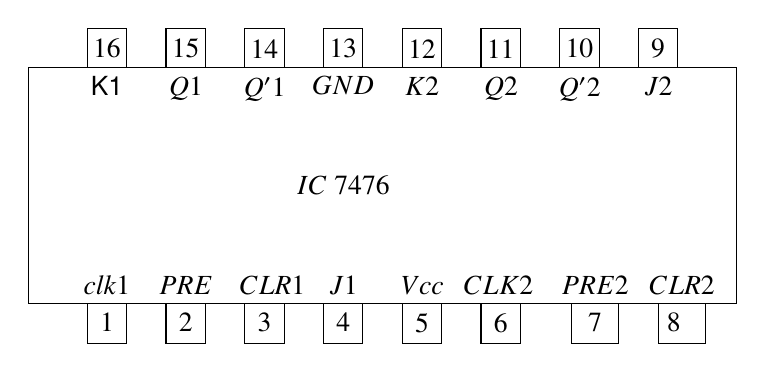
\begin{tikzpicture}
    \draw (0,2) rectangle (9,5);
    \draw (4,3.5) node{$IC$ $7476$};
    \draw (0.75,2) rectangle(1.25,1.5);
    \draw (1,2) node[below]{$1$};
    \draw (1,2) node[above]{$clk1$};
    \draw (1.75,2) rectangle (2.25,1.5);
    \draw (2,2) node[below]{$2$};
    \draw (2,2) node[above]{$PRE$};
    \draw (2.75,2) rectangle (3.25,1.5);
    \draw (3,2) node[below]{$3$};
    \draw (3.1,2) node[above]{$CLR1$};
    \draw (3.75,2) rectangle (4.25,1.5);
    \draw (4,2) node[below]{$4$};
    \draw (4,2) node[above]{$J1$};
    \draw (4.75,2) rectangle (5.25,1.5);
    \draw (5,2) node[below]{$5$};
    \draw (5,2) node[above]{$Vcc$};
    \draw (5.75,2) rectangle (6.25,1.5);
    \draw (6,2) node[below]{$6$};
    \draw (5.97,2) node[above]{$CLK2$};
    \draw (6.9,2) rectangle (7.5,1.5); % block of pin 7
    \draw (7.2,2) node[below]{$7$};
    \draw (7.2,2) node[above]{$PRE2$};
    \draw (8,2) rectangle (8.6,1.5); %block of pin 8
    \draw (8.2,2) node[below]{$8$};
    \draw (8.3,2) node[above]{$CLR2$};
    \draw (0.75,5) rectangle (1.25,5.5);% block of pin 16
    \draw (1,5) node[above]{$16$};
    \draw (1,5) node[below]{K1};
    \draw (1.75,5) rectangle (2.25,5.5);
    \draw (2,5) node[above]{$15$};
    \draw (2,5) node[below]{$Q1$};
    \draw (2.75,5) rectangle (3.25,5.5);
    \draw (3,5) node[above]{$14$};
    \draw (3,5) node[below]{$Q'1$};
    \draw (3.75,5) rectangle (4.25,5.5);
    \draw (4,5) node[above]{$13$};
    \draw (4,5) node[below]{$GND$};
    \draw (4.75,5) rectangle (5.25,5.5);
    \draw (5,5) node[above]{$12$};
    \draw (5,5) node[below]{$K2$};
    \draw (5.75,5) rectangle (6.25,5.5);
    \draw (6,5) node[above]{$11$};
    \draw (6,5) node[below]{$Q2$};
    \draw (6.75,5) rectangle (7.25,5.5);
    \draw (7,5) node[above]{$10$};
    \draw (7,5) node[below]{$Q'2$};
    \draw (7.75,5) rectangle (8.25,5.5);
    \draw (8,5) node[above]{$9$};
    \draw (8,5) node[below]{$J2$};
\end{tikzpicture}

	\label{pindiagram.}
\end{center}
\section{Implementation}
The connections between Arduino UNO and three IC 7476 is given in below Table \\
\begin{table}[h]
  \begin{center}
  \begin{tabular}{|c|c|c|c|c|c|c|c|c|c|c|}
    \hline & \multicolumn{2}{|c|}{INPUT} & OUTPUT & CLOCK 1 & clock 2 & Vcc & GND \\
    \hline ARDUINO & D2 & D3 &   &  13 &    & 5V & Gnd  \\
    \hline 7476 & \multicolumn{1}{|c|}{16,2,3} & \multicolumn{1}{|c|}{} & \multicolumn{1}{|c|}{15} & 1 & 15 & 5 & 13 \\
    \hline 7476 & \multicolumn{1}{|c|}{} & \multicolumn{1}{|c|}{16} &  15 &  & 1 & 5 & 13 \\
            \hline
  \end{tabular}
  \end{center}
  \caption{connections}
  \label{table:1}
\end{table}
\section{Procedure}
\begin{raggedright}
    1.Connect the circuit as per the above table.\\
    2.connect the output pins to the LED's \\
    3.Connect inputs to Vcc for logic 1,ground for logic 0 \\
    4.Execute the circuit using the below code.\\
\begin{table}[h]
\centering
  \begin{tabular}{|c|}
  \hline
   https://github.com/Goutham-patel/\\
	  FWC/blob/main/ide/codes/src/In201912.cpp\\
  \hline
\end{tabular}
\end{table}
\end{raggedright}
\bibliographystyle{article}


\end{document}
